\chapter{Project}
In this bachelor thesis the KIT-Dataset\cite{Plappert2016} will be used to train classifiers of human motions with classes such as walk, run and dance. The KIT contains a number of motions and the relevant information to simulate and classify these motions. The raw dataset can be divided into 4 components:
\begin{itemize}
	\item The motions themselves, in mmm-Notation in xml-files as outlined in \ref{subsec:mmm-notation}.
	\item The motions in the c3d-Notation in c3d-files. These files wont be used in this project.
	\item Annotations of each motion, outlining the activity performed in the recorded motion. These annotation are persistently stored as json-files.
	\item Meta information for each motion, which are irrelevant for this project.
\end{itemize}
The goal of this project is to extract the necessary information out of each motion mmm-file and generate a classification for each motion based on the corresponding motion file. Then to used to train leaning machines to predict the class of the motion.
\section{Dataset}
\begin{wrapfigure}{R}{.4\textwidth}
	\vspace{-1.5cm}
	\begin{center}
		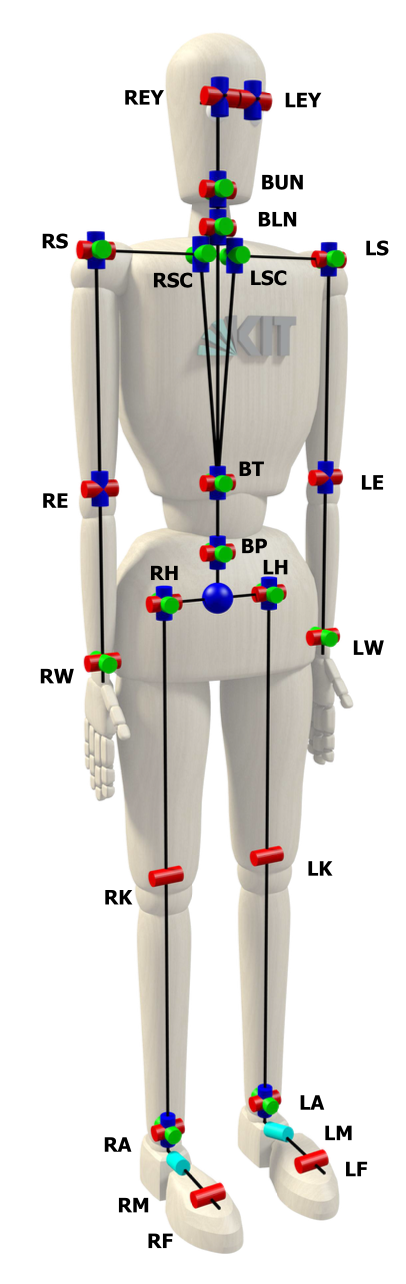
\includegraphics[width=.25\textwidth]{img/mmm-model.png}
		\caption{The base of the mmm model as in \cite{Plappert2016}}
		\label{fig:mmm-model}
	\end{center}
\end{wrapfigure}
As mentioned in the introductory part of this chapter, the KIT-Motion dataset\cite{Plappert2016} will be used, and in this section the relevant information about the dataset will be discussed. This dataset was first assembled to link human motions to the natural language, which is of huge interest for the generation of semantic presentations of human activities. In addition to that, this dataset would be instrumental in implementing leaning machines capable of generating robot activities based on natural language input\cite{Plappert2016}. The team responsible of KIT Motion Database has developed the tools to aggregate the data from multiple motion capture databases and included the results in their database using a unified representation outlined in \ref{subsec:mmm-notation}. According to the team the dataset contains a total of 3911 motions totaling 11.23 hours motion capturing duration\cite{Plappert2016}.
\subsection{mmm-Notation} \label{subsec:mmm-notation}
The information about the motions in this dataset are persistently stored as xml-files using the mmm-notation ensuring the ease of reusability and the portability of these files. For this notation the mmm(Master Motor Map) was developed which is a framework and toolkit for capturing, representing and reproducing human motion. In this thesis only the representing part is relevant for extracting the information about the position of the joints the velocity and the root joint position for example\cite{mmm2014}. The xml-based mmm-notation is made of two parts. First, the setup on the model with the necessary information to recreate the motion itself, such as the height and the mass of the human, which are stored in the xml-element \texttt{ModelProcessorConfig}. In addition to that the joints are defined in the xml-element \texttt{JointOrder} and its child elements. Relevant here are the motion frames stored as \texttt{MotionFrames}, where the informations about the frames of the motions are stored as the children the \texttt{MotionFrames} xml-element:
\begin{itemize}
	\item The time step of the frame in \texttt{Timestep} xml-element.
	\item The root joint positions in each frame in the \texttt{RootPosition} xml-element.
	\item The root rotations in each frame in the \texttt{RootRotation} xml-element.
	\item Information about the joints sorted according to the joint order specified in the \texttt{JointOrder} xml-element, and these joints are illustrated in fig \ref{fig:mmm-model}
	\begin{itemize}
		\item The position of each joint in \texttt{rad} in the \texttt{JointPosition} xml-element.
		\item Analog to the \texttt{JointPosition} xml-element the velocity of each joint is stored in the \texttt{JointVelocity} xml-element.
		\item And lastly for the joint acceleration of each joint in the \\\texttt{JointAcceleration} xml-element.
	\end{itemize}
\end{itemize}
To extract the information stored in these xml-files, the \texttt{python} library \\\texttt{xml.etree.ElementTree} is used to parse the files. With it the xml-file is parsed and converted into a tree, that can be navigated through iterating over the xml-children of each xml-element until the necessary information is found and extracted either as an attribute of an element or the body of it. These can be ascertained using the \texttt{get} or the \texttt{text} methods. 
\subsection{Motion labeling}
As mentioned in the introductory part of this section, the KIT provided annotations to each motion in this dataset. These annotation are the base for the labeling of each motion, as a class describing and representing the motion as a whole and not describing it in details. These annotation are a list of sentences describing the motion in multiple turn of phrases. This is useful for generating of semantic presentations of human activities, bus is irrelevant here. Thus, the natural language processing library \texttt{nltk} was used to process these annotations and extract the verbs and classifying them by the frequency of their occurrences. The position tagging was achieved by using the average perceptron, which theoretical foundation was outlined in \ref{subsec:wordtaggers}. Then, the most frequent verbs are determined and used as labels to the motions where they are part of the assigned annotation. Some verbs, such as be and so..., are for this task marked as stop verbs and discarded. The resulted list of most frequent verbs is \{'walk', 'turn', 'run', 'stand', 'jump', 'wave', 'stumbl', 'danc', 'throw', 'kneel', 'kick'\}. However, the use of stemer, as explained in \ref{subsec:stemmer}, is paramount to correctly estimate the frequency and to uniformly classify motion, without taking into account the tense and the position of the verb in the annotation. In this thesis, the snowball stemmer was used to determine the stem of each verb encountered in all annotations. Lastly, each motion was labeled by the stem of a verb by iterating over the tokens in the annotation and searching for a verb in the most frequent list of verbs calculated beforehand.
\subsection{Preliminary Analysis}
To asses the usefulness of the dataset the library \texttt{Bokeh} some statistical analysis of the dataset must be done. First, the number of motions without annotations must be determined and the affected motions must be discarded. By implementing a downloader object, that extracts the content of the zip file containing the files. Then, the annotations will be checked and determined, if these are empty. A total of 3012 motions were correctly annotated, and the rest was deleted.\newline
The motions vary in length and the number of frames of them, and in \ref{section:training} some sequential models were used to train the models implemented in \ref{section:leaningmachines}, thus the length of the frames must be defined to both ensure taking all the relevant information for the classification and avoid padding the motions too much with zeros. As the number of frames to be feet to the model to generate a prediction of to train it must have a beforehand defined length. The distribution of the number of frame for all motion is visualised in fig \ref{fig:num_frames_distro}. In addition to that, fig \ref{fig:scatterplot-num-frames} displays a scatter plot of the number of frames in the motions. Taking the results of the visualisation into account, it has been determined that the length of the most motions is around 2000 frames. Thus, this value has been chosen to be the standard input length in \ref{section:learningmachines}.
\begin{figure}
	\centering
	\begin{subfigure}[b]{0.47\textwidth}
		\centering
		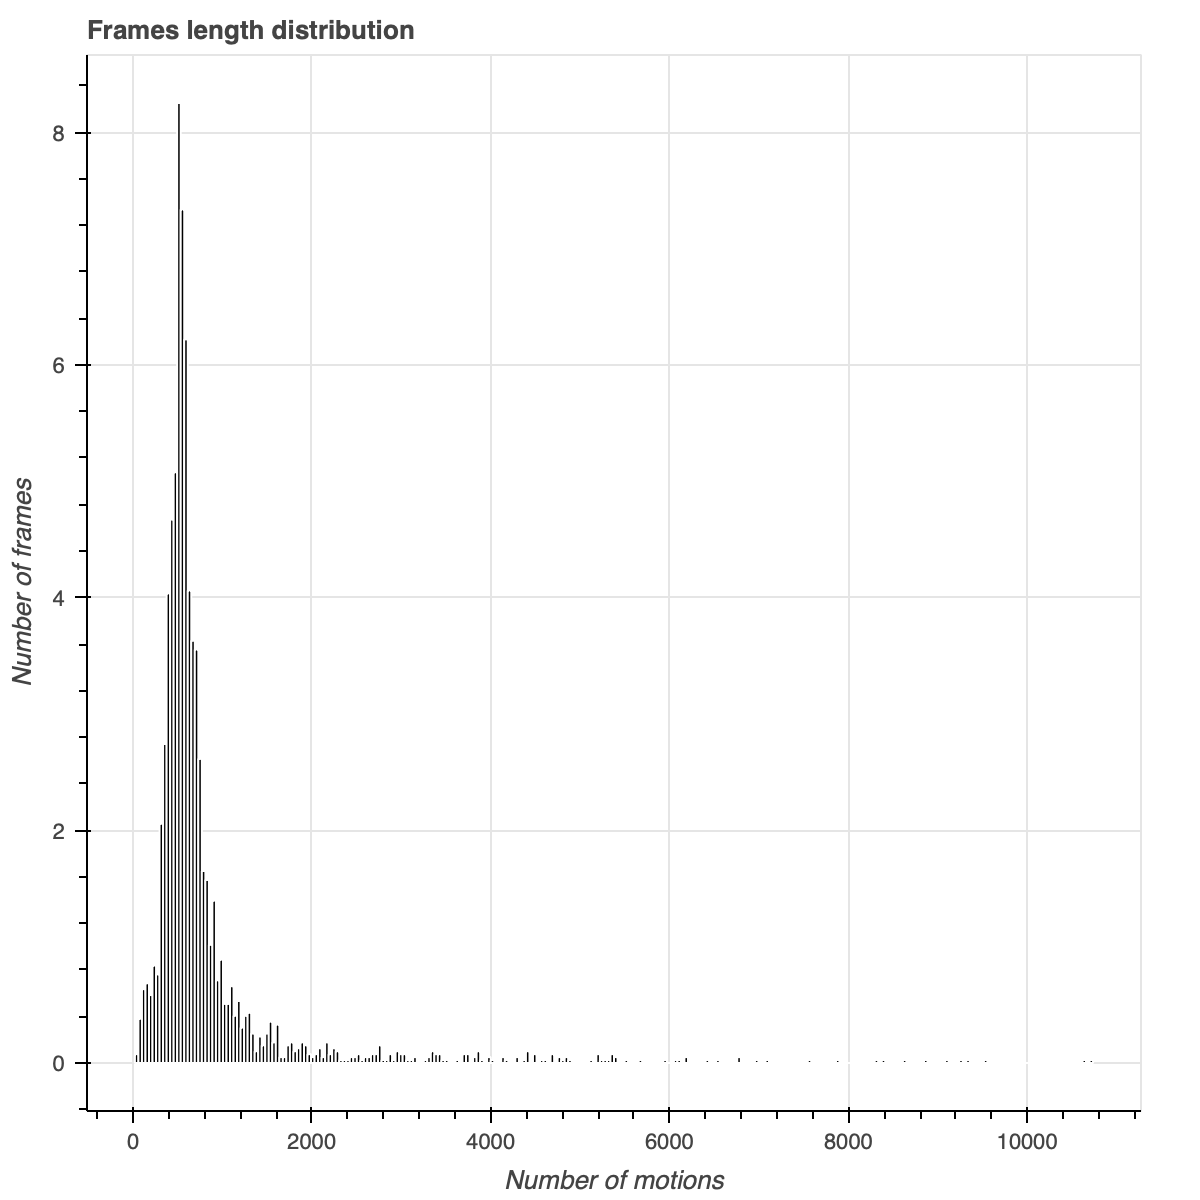
\includegraphics[width=\textwidth]{img/num-frames-ditro.png}
		\caption{The distribution of the number of frames over all the motions}
		\label{fig:num_frames_distro}
	\end{subfigure}
	\hfill
	\begin{subfigure}[b]{0.47\textwidth}
		\centering
		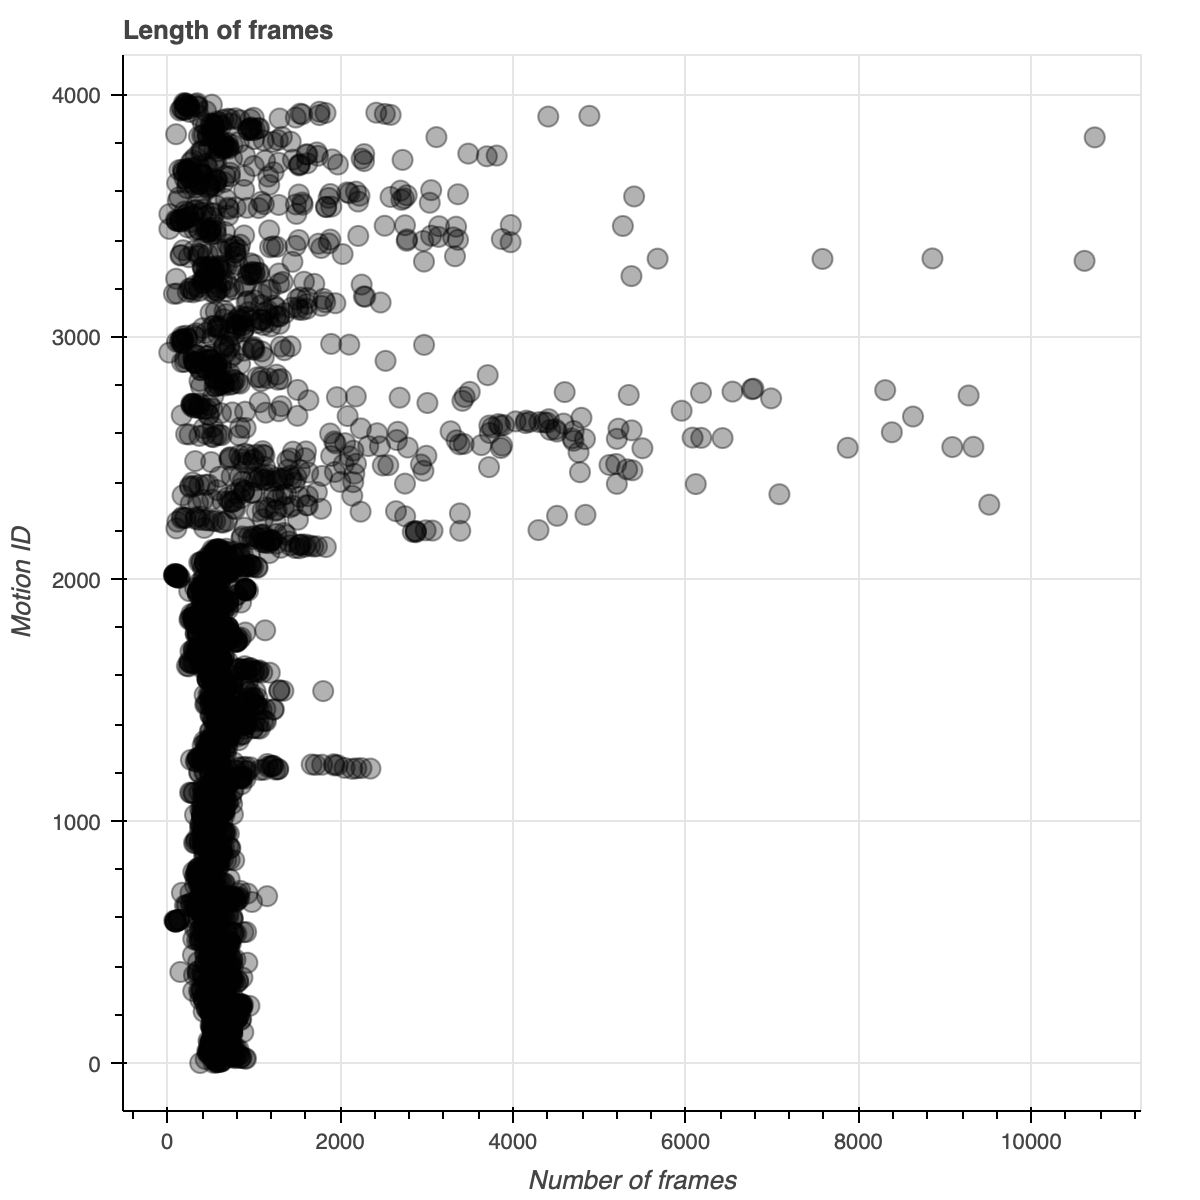
\includegraphics[width=\textwidth]{img/scatter-num-frames.png}
		\caption{The scatter plot for the lengths of motions}
		\label{fig:scatterplot-num-frames}
	\end{subfigure}
\end{figure}
In addition to that, it has been shown that all the \texttt{JointVelocity} and \texttt{JointAcceleration} xml-element are all not defined and 0. This making them irrelevant for this project. In section \ref{section:leaningmachines}, only the information stored in \texttt{JointPosition}, \texttt{RootPosition} and \texttt{RootRotation} will be extracted and used in the next steps.
\section{Learning Machines}
\label{section:leaningmachines}
For the propose of training and evaluating the results of each leaning machine used in this thesis. The MLP(Multilayer Perceptron) and the CNN(Convolutional Neural Network) have been used as a base line to be compared to. At first, it was assumed that dedicated model for sequential input, such as RNN(Recurrent Neural Networks), GRU(Gated Recurrent Units) and LSTM(Long Short Term Memory), would prove more performant than the base line, but this was in most cases not true. In this section, the implementation of the used learning machines will be discussed in further details. To achieve this the machine learning \texttt{pytorch} was used, as it offers a well documented and accessible library suitable for the goals and aspiration of this thesis. To experiment with models, the implementation should be flexible, as in the number of features could vary according to the number of features extracted. The implementation of the extraction of the information about the frames of a motion is done with the following three cases:
\begin{enumerate}
	\item Extracting only the information about the root joint, i.e. the rotation and the position in space.
	\item Extracting only the information about the joints, i.e. the rotation of each joint on an axis.
	\item Extracting all the information available in the xml-files.
\end{enumerate}
The result is a sequence of vectors containing the information, that is then used to train the model or to generate a prediction.\newline
First, a very simple MLP(Multilayer Perceptron) was implemented. To experiment with it, it has been trained using the three cases as outlined before. This will demonstrate, if the models would perform better with more features. The architecture of the model is illustrated in fig. \ref{fig:wang2017timemlp}. As a base line, a CNN(Convolutional Neural Network) was also used. These models proved to be good varying degrees, and the results of their training will be discussed in \ref{sec:evaluation}. Next, more suitable models for the 
% TODO: Explain the recurrent models used and add illustration of them, based on the theoretical past of this thesis
\section{Training}\label{section:training}
Now, the models can be trained, but a inherent problem of HAR(Human Activity Recognition) comes to light as outlined in \ref{subsec:probHAR}
\section{Evaluation}\label{sec:evaluation}
\section{Verbesserungsvorschläge}
